%        File: report.tex
%     Created: Sat Nov 03 06:00 PM 2018 E
% Last Change: Sat Nov 03 06:00 PM 2018 E
%
\documentclass[a4paper]{article}
\usepackage{graphicx}
\usepackage{hyperref}
\usepackage[noabbrev,capitalise]{cleveref}
\usepackage{natbib}

\begin{document}

\title{Baby Name Popularity}
\author{
Francisco Rivera \\ \texttt{frivera@college.harvard.edu}
\and
Mark Chamberlain}

\maketitle

\begin{abstract}
The U.S. Census publishes the number of babies born to each first name each year
at the country and state level. These trends exhibit dramatic up- and
down-swings unexplainable by a simple imitation model. We attempt to construct a
model to explain the dynamics of these popularity swings as well as other
stylized facts from the data.
\end{abstract}

\section{The Data}

Our data comes from the U.S.
Census.\footnote{\url{https://catalog.data.gov/dataset/baby-names-from-social-security-card-applications-national-level-data}}
The dataset allows us to observe the number of births in the country each year
by first name and gender with the exception of names for which there were fewer
than five births.

The data requires little processing, but because our aim is to model changes in
popularity rather than population growth, we normalize each data entry as a
percentage of the total number of births that year. To provide a sense of what
some typical trends look like, we plot the popularity of five random
popular\footnote{Defined as exceeding 0.5\% of all births on any year.} names in
\cref{fig:fivenames}.

\begin{figure}[h]
\centering
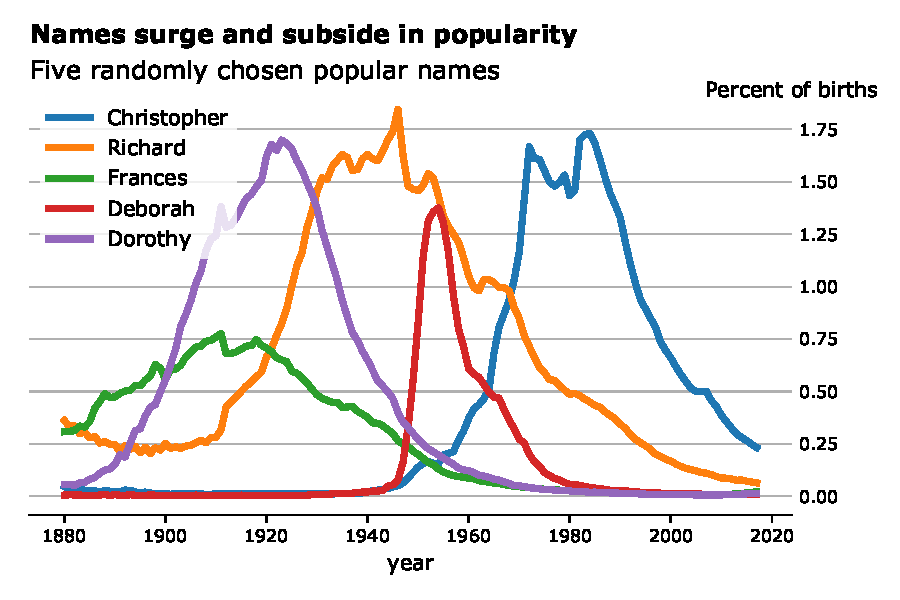
\includegraphics[width=.9\textwidth]{figs/five-rand-names}
\caption{Popularity evolution of five random names}
\label{fig:fivenames}
\end{figure}

On the basis of inspecting many realizations of \cref{fig:fivenames}, for which
the depicted trends are representative, we can take away some stylized facts,

\begin{itemize}
\item The popularity of a name in many cases follows a exponential-like growth
from obscurity, a peak, and then a decay back to obscurity.
\item There appears to be a practical upper-bound to how high the peak is, but
this upper bound need not be binding for many names
\item As ``Deborah'' shows, the down-swing need not be as fast as the up-swing.
\end{itemize}

\section{An Imitation Model}

We will follow \cite{hahn2003drift} closely.

\section{Segmenting the population}

\bibliography{sources}
\bibliographystyle{apalike}

\end{document}


